\section{Motivation}
\label{sec:motivation}

Memory is a critical type of resource in current data processing systems, especially in the in-memory computing systems~\cite{shi:mammoth}. Limited memory space leads to memory pressure and can cause frequent garbage collection or out-of-memory errors~\cite{fang2015interruptible}, both of which seriously affect the performance of the data processing system. A data processing system is often deployed as a batch processing system, but can also be deployed as a service and work as a service-oriented system. 

To understand the impact of memory pressure on the service-oriented data processing systems and identify the cause of inefficiency, we investigate different applications in Spark. Spark can also work as a service-oriented system through the Spark Job Server. We choose two types of applications, PageRank(PR)  which is a typical benchmark in Spark, and Aggregation Query(AQ) which is the common big data benchmarks in SQL~\cite{www:benchmark}. In order to stand for a general situation, a semantic-identical hand-written Spark program are used for AQ. The input dataset of PR and AQ are webbase-2001 (30GB) and HiBench Random Writer (50GB).  We first run the tasks in the service-oriented mode, in which we submit PR and AQ simultaneously to the service-oriented Spark and run them with a fair scheduler in Spark. As a comparison, we also run PR and AQ in the batch mode, in which PR and AQ are processed one after the other. We record the execution times and garbage collection times of all tasks under these two modes, which are plotted in Figure~\ref{fig:memorypressure}. We then analyze the  memory pressure through the results.   

\begin{figure}[!t]
\centering
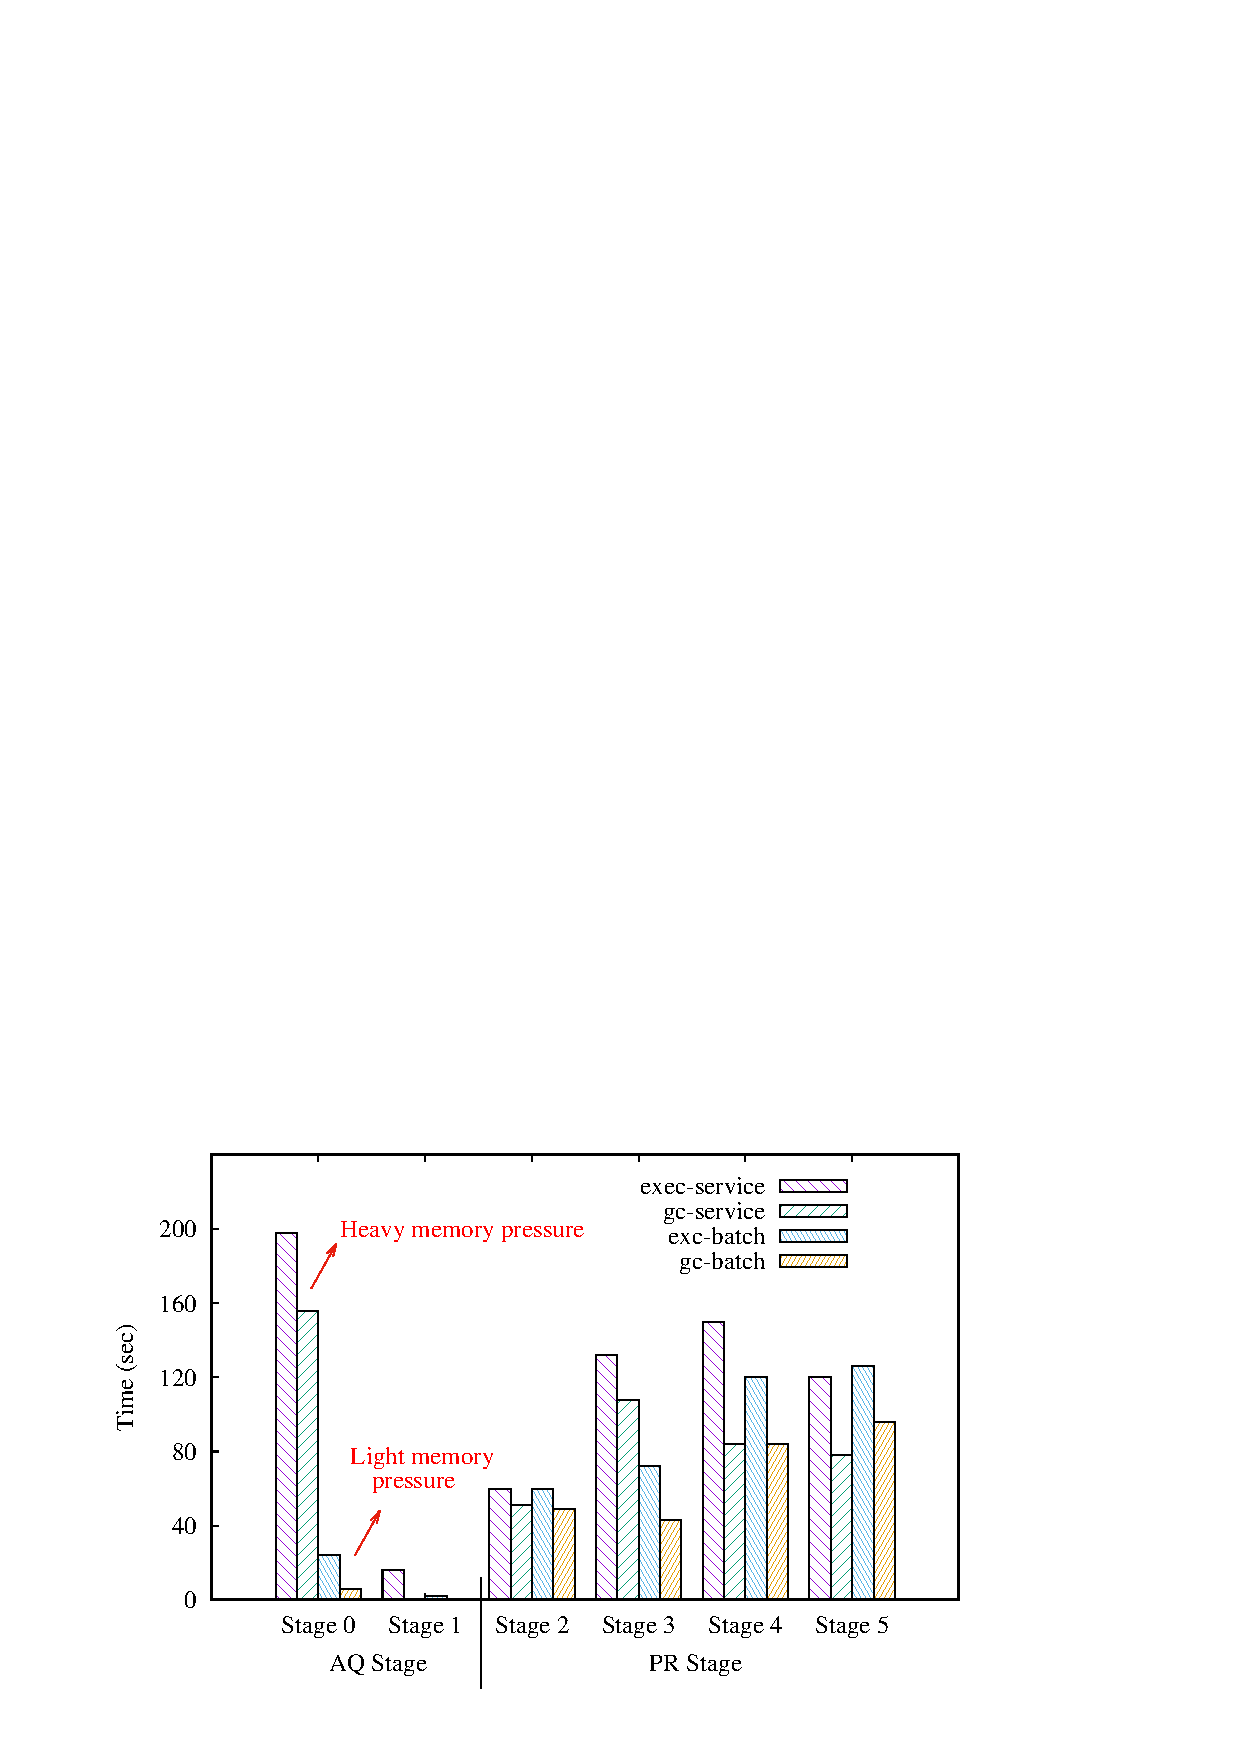
\includegraphics[width=0.35\textwidth]{motivation-exec-gc.pdf}
\vspace{-2mm}
\caption{AQ suffers memory pressure from PR}
\vspace{-6mm}
\label{fig:memorypressure}
\end{figure}

We observe that PR caches intermediate data in memory and iteratively compute the result. One iteration corresponds to one stage in Spark. Because the caching data is alive as long as the job itself, the memory space becomes gradually less and the task computation will suffer. If this occurs, it indicates the memory pressure caused by PR is heavy. Compare with PR, however, AQ only contains some simple operations. AQ has only two processing stages and during its execution, a very small amount of intermediate shuffle data are generated (although the input data of AQ is larger than that of PR). Furthermore, both the execution time and garbage collection time are low in AQ, and the memory pressure is much lighter than PR. The result of PR in the batch mode also verifies its high memory pressure and heavy garbage collection, which are the results labelled as exec-batch and gc-batch in Figure~\ref{fig:memorypressure}. As we can see, the garbage collection time accounts for a very large proportion of the execution time.

When multiple jobs, such as PR and AQ, are submitted to and run by the Spark service simultaneously, the jobs are run with a fair scheduler provided by Spark. Although AQ has much more light memory pressure  than PR, all running tasks suffer from the heavy memory pressure produced by PR. We find that the execution time (exec-service in Figure~\ref{fig:memorypressure} of every task in each stage of PR has little change, except some maximum execution times. This is because almost all memory pressure comes from PR and therefore the executions of PR in the service mode and the batch mode show similar trends. However, The execution of AQ in the service mode is very different from that in the batch mode. This is because in the service mode, both applications are run simultaneously and therefore AQ suffers from the memory pressure produced by PR even if AQ is a light task itself. In the batch mode, since the applications are run one after another. The high memory pressure created by PR will not affect the running of AQ.

In summary, our results implicate that in a service-oriented system, 1) the heavy memory pressure will result in frequent garbage collection, which consumes most of the time and reduces the throughput; 2) the light tasks suffer from heavy memory pressure produced by the heavy tasks; and 3) the heavy tasks obtain the resources later because these resources are occupied chronically by light tasks, and the heavy tasks themselves are the source of memory pressure.

By observing the first stage of PR and AQ, we discover that the tasks of PR and AQ invoke different function APIs, which determine the impact of each task on memory pressure. If we can identify and classify these tasks by the characteristics of the function APIs, we can suspend the heavy tasks and leave adequate memory space to the light tasks when the memory pressure shows up. This can improve the throughput of the service-oriented systems and allow all tasks to run with enough memory space and hence light memory pressure. 
  
